\documentclass{standalone}
\usepackage{tikz}
\usetikzlibrary{positioning, shapes.geometric, arrows.meta}

\begin{document}
	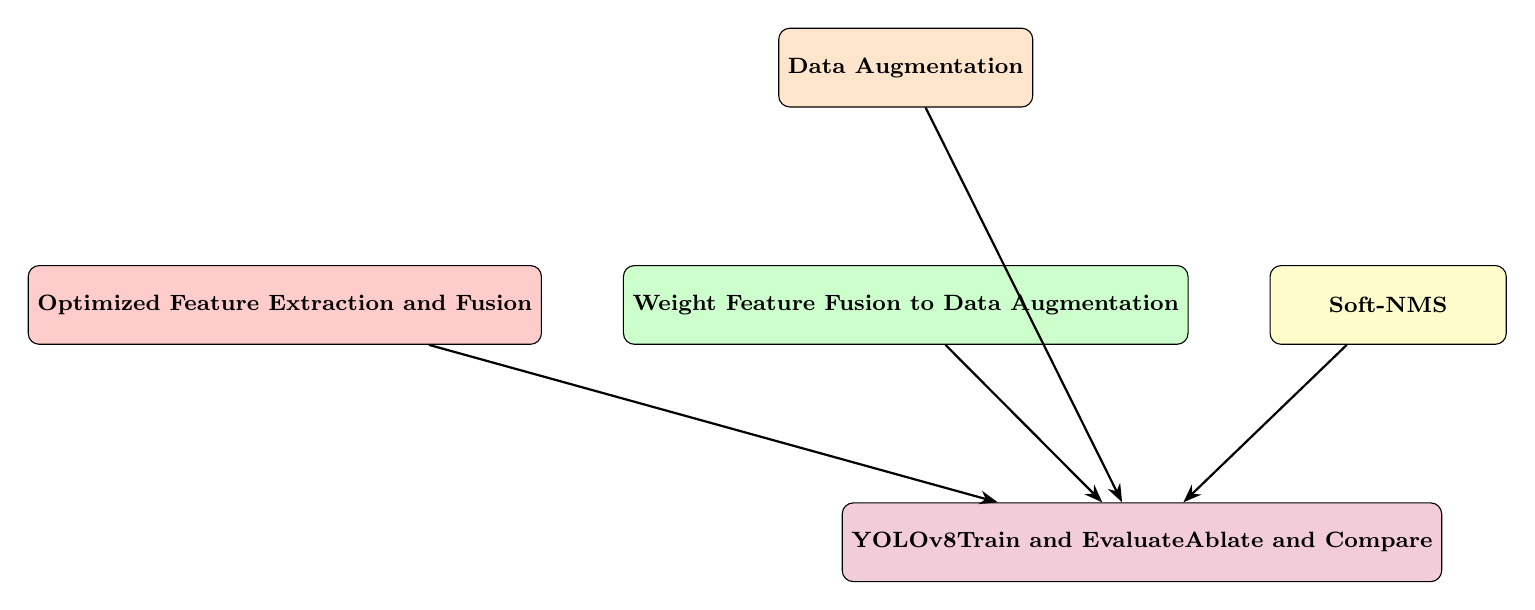
\begin{tikzpicture}[
		node distance=2cm and 3cm,
		box/.style={rectangle, draw, rounded corners, minimum width=3cm, minimum height=1cm, font=\bfseries\footnotesize, fill=blue!20},
		arrow/.style={thick,->,>=Stealth}
		]
		
		% Nodes
		\node[box, fill=orange!20] (A) {Data Augmentation};
		\node[box, fill=yellow!20, below right=of A] (B) {Soft-NMS};
		\node[box, fill=green!20, below=of A] (C) {Weight Feature Fusion to Data Augmentation};
		\node[box, fill=red!20, below left=of A] (D) {Optimized Feature Extraction and Fusion};
		\node[box, fill=purple!20, below=of C, xshift=3cm] (E) {YOLOv8\\Train and Evaluate\\Ablate and Compare};
		
		% Edges
		\draw[arrow] (A) -- (E);
		\draw[arrow] (B) -- (E);
		\draw[arrow] (C) -- (E);
		\draw[arrow] (D) -- (E);
		
		% Optionally, add more styling or elements to enhance aesthetics
		% For example, background rectangles for groups of nodes
		
	\end{tikzpicture}
\end{document}
